%%%%%%%%%%%%%%%%%%%%%%%%%%%%%%%%%%%%%%%%%%%%%%%%%%%%%%%%%%%%%%%%%%%%%%%%%%%%%%%
%
% Introduction
% Copyright (c) 2010 by tilo.mueller@rwth-aachen.de
% 
%%%%%%%%%%%%%%%%%%%%%%%%%%%%%%%%%%%%%%%%%%%%%%%%%%%%%%%%%%%%%%%%%%%%%%%%%%%%%%%

\chapter{Einführung}

%Section		Depth
%\part			1
%\chapter		2
%\section 		3
%\subsection 		4
%\subsubsection 	5 	-> from here on it's not in default TOC anymore
%\paragraph	 	6
%\subparagraph 		7

\section{Motivation}
Mit den vor kurzem aufgetretenen Veröffentlichungen durch Edward Snowden sind der Datenschutz und die Privatsphäre wieder zu einem relevanten Gesprächsthema geworden. So sagt zum Beispiel Hanspeter Thür, der Datenschutzbeauftragte der Schweiz: "Privatsphäre wird zu einem Privileg" \cite{nzzdatenschutzprivileg}. Durch diese Debatten geraten auch große Unternehmen im Internet wieder in den Fokus. Da auch in Deutschland die Google Inc. eine sehr große Nutzerbasis hat (alleine in Deutschland nutzen ungefähr 38 Millionen Nutzer die Suchmaschine von Google \cite{statistagoogle}), ist es logisch, dass auch sie des öfteren mit Datenschützern in Konflikt gerät (siehe zum Beispiel "Datenschützer: Google verstößt gegen geltendes Recht" \cite{gulligooglegeltendesrecht}). Die Google Suchmaschine ist dabei nicht der einzige Google Dienst der dabei in den Mittelpunkt von Diskussionen gerät. Spätestens seit Julian Assange Google eine "privatisierte NSA" genannt hat \cite{assangegooglensa}, ist es klar, dass man sich im Bezug auf persönliche Daten bei Google besonders Gedanken machen muss.\\
Dabei ist der wichtigste Aspekt der Mensch selbst - und zwar nicht die Mitarbeiter von Google oder die Datenschützer im Besonderen sondern die normalen Nutzer. Der Nutzer ist derjenige, dessen Daten von Google verwendet werden und somit derjenige der sich davor Schützen kann, oder damit leben muss dass Google die Daten besitzt.


\section{Zielsetzung und Forschungsfragen}
Diese Arbeit soll die Nutzer von Google näher betrachten und herausfinden wie diese Nutzer über ihren Datenschutz im Bezug auf Google denken und wie sie vorgehen um ihre Daten zu schützen. Hierzu wird eine Umfrage durchgeführt die Nutzer über ihr Verhalten auf Google und ihre Gedanken über Google befragt.
Die grundsätzlichen Forschungsfragen die behandelt werden sind "Wie viel wissen Nutzer von der Datensammlung durch Google?" und "Versuchen sie gegen dieses Sammeln von Daten vorzugehen?". 

\section{Kategorien zur Einordnung der Fragen}
\label{sec:categories}
Zum Aufstellen der Hypothesen und zur späteren Einteilung der Fragen des Fragebogens wurden Kategorien aufgestellt, die wie folgt definiert wurden:
\begin{enumerate}
\setcounter{enumi}{-1}
\item \label{itm:Kat0}\textbf{Nutzung von Google Diensten}: Das Nutzungsverhalten der Google Dienste von Seiten der Nutzer. Dieser Teil fragt vor allem allgemeine Daten zum Nutzungsverhalten ab. Darunter fallen unter anderem die Information, welche Dienste genutzt werden und wie viele Accounts die Nutzer haben.
\item \label{itm:Kat1}\textbf{Kenntnisse über Googles Datenschutz}: Angeeignetes Wissen über den Umgang mit personenbezogenen Daten bei Google, vor allem im Bezug auf die genutzten Dienste. Hierbei sind Fragen wie "Bietet Google auf Nutzer zugeschnittene Werbung an?" relevant.
\item \label{itm:Kat2}\textbf{Vertrauen in Google}: Das Glauben an auftrende negative Konsequenzen im Zusammenhang mit dem Preisgeben der Daten (vgl. Kim et al., 2008).
\item \label{itm:Kat3}\textbf{Wahrgenommenes Risiko für die Privatsphäre}: Das Glauben an auftretende negative Konsequenzen im Zusammenhang mit dem Preisgeben der Daten (vgl. Kim et al., 2008)
\item \label{itm:Kat4}\textbf{Aufgeben der Privatsphäre}: Das Bewusstsein über den Verlust der Privatsphäre bei der Verwendung von Google Diensten.
\item \label{itm:Kat5}\textbf{Schutzmaßnahmen}: Verhalten des Nutzers zum Schutze der eigenen Privatsphäre
\end{enumerate}

\section{Hypothesen}
Die Forschungsfragen werden beantwortet indem Hypothesen aufgestellt werden die den Zusammenhang der oben genannten Kategorien darstellen.
Die Hypothesen sind angetragen, indem zuerst die beiden Kategorien aufgelistet werden, zwischen denen die Hypothese einen Zusammenhang darstellen soll. Danach kommt eine kurze Definition der Hypothese.
Die zugehörigen zu testenden Hypothesen sind die Folgenden:
\begin{description}
\item[\label{itm:H0}\textbf{H0}] Nutzung von Google Diensten \ref{itm:Kat0} $\rightarrow$ Kenntnisse über Googles Datenschutz \ref{itm:Kat1}: Wenn eine Person Google aktiver nutzt, bekommt sie mehr Erfahrung und Kenntnisse über Google Dienste und mögliche Probleme mit der Privatsphäre
\item[\label{itm:H1}\textbf{H1}] Kenntnisse über Google \ref{itm:Kat1} $\rightarrow$ Aufgeben der Privatsphäre \ref{itm:Kat4}: Je mehr eine Person über Googles Datenschutz weiß, desto seltener gibt sie Teile ihrer Privatsphäre auf
\item[\label{itm:H2}\textbf{H2}] Vertrauen in Google \ref{itm:Kat2} $\rightarrow$ Wahrgenommenes Risiko für Privatsphäre \ref{itm:Kat3}: Je höher das Vertrauen in Google ist, desto geringer wird das Risiko eingeschätzt.
\item[\label{itm:H3}\textbf{H3}] Wahrgenommes Risiko für Privatsphäre \ref{itm:Kat3} $\rightarrow$ Schutzmaßnahmen \ref{itm:Kat5}: Je höher das Risiko eingeschätzt wird, desto mehr Schutzmaßnahmen werden unternommen.
\item[\label{itm:H4}\textbf{H4}] Schutzmaßnahmen \ref{itm:Kat5} $\rightarrow$ Aufgeben der Privatsphäre \ref{itm:Kat4}: Wenn eine Person mehr Schutzmaßnahmen verwendet, dann gibt sie weniger Teile ihrer Privatsphäre auf.
\end{description}
Durch die Umfrage sollen diese Hypothesen belegt oder widerlegt werden und somit die Zusammenhänge dargestellt und letzten Endes die Forschungsfrage beantwortet werden.

Der Zusammenhang zwischen den Kategorien und den Hypothesen soll anhand folgender Grafik verdeutlicht werden:
\begin{figure}[H]
\centering
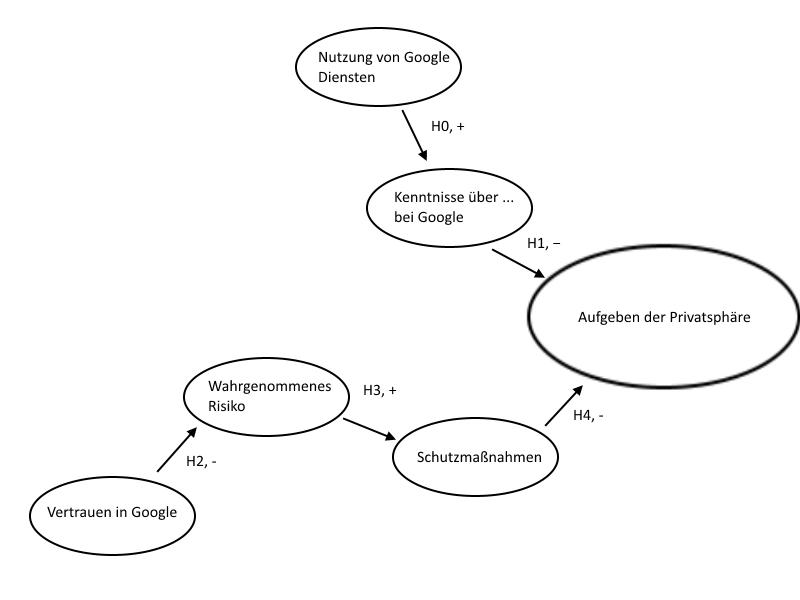
\includegraphics[scale=0.55]{images/bubbles}\\
\caption{Zusammenhang zwischen Kategorien und Hypothesen}\label{bubbles}
\end{figure}